\documentclass{standalone}
\usepackage{tikz}
\usepackage{color}
\usepackage{caption}
\usepackage{amssymb}
\colorlet{blueteal}{blue!50!teal}
\colorlet{greenish}{green!50!cyan}
\begin{document}
\centering
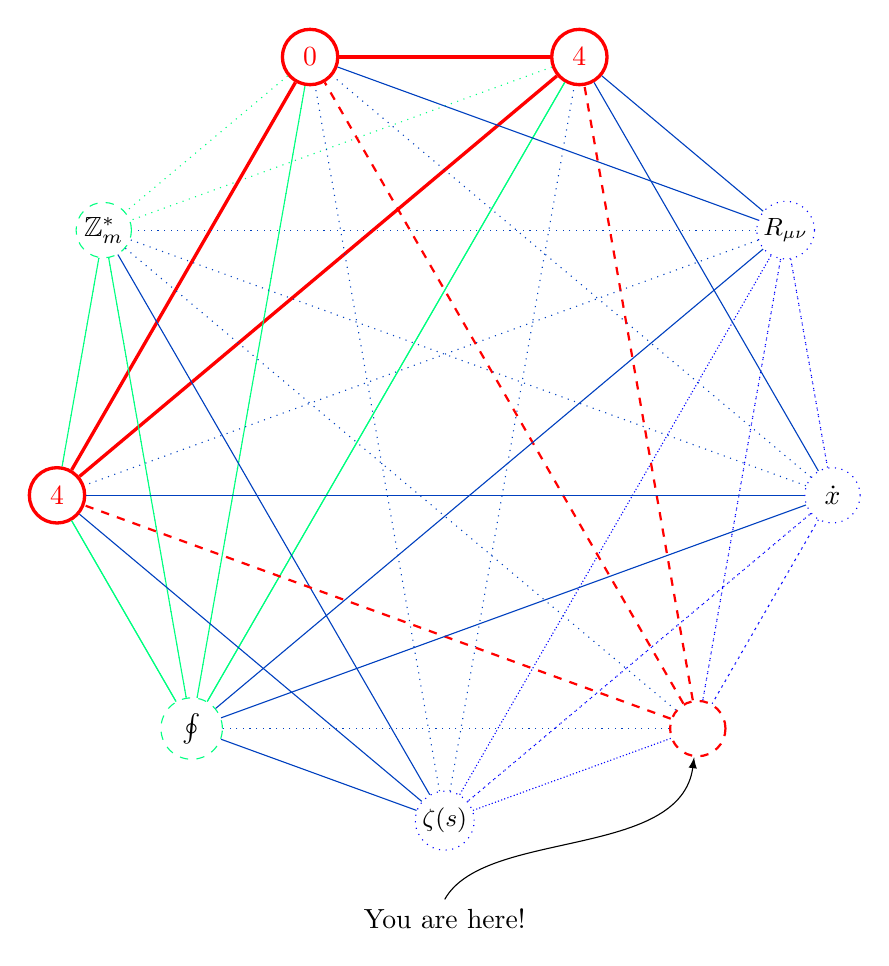
\begin{tikzpicture}
\node[circle, draw=blue,thin,  dotted, minimum size = 2em, inner sep=1pt] (0) at (-9.184850993605148e-16, -5.0) {\small$\zeta(s)$};
\node[circle, draw=red, thick, dashed, minimum size = 2em, inner sep=1pt] (1) at (3.2139380484326963, -3.8302222155948904) {};
\node[circle, draw=blue,thin,  dotted, minimum size = 2em] (2) at (4.92403876506104, -0.8682408883346564) {$\dot{x}$};
\node[circle, draw=blue,thin,  dotted, minimum size = 2em, inner sep=1pt] (3) at (4.330127018922195, 2.4999999999999964) {\small$R_{\mu\nu}$};
\node[circle, draw=red, very thick, minimum size = 2em] (4) at (1.7101007166283433, 4.698463103929543) {\color{red}4};
\node[circle, draw=red, very thick, minimum size = 2em] (5) at (-1.7101007166283402, 4.6984631039295435) {\color{red}0};
\node[circle, draw=greenish, thin, dashed, minimum size = 2em, inner sep=1pt] (6) at (-4.330127018922189, 2.5000000000000067) {$\mathbb{Z}^*_m$};
\node[circle, draw=red, very thick, minimum size = 2em] (7) at (-4.924038765061041, -0.8682408883346489) {\color{red}4};
\node[circle, draw=greenish, thin, dashed, minimum size = 2em] (8) at (-3.213938048432695, -3.8302222155948913) {$\oint$};
\draw[blue, dotted] (0) -- (0);
\draw[blue, dotted] (0) -- (1);
\draw[blue, dotted] (0) -- (2);
\draw[blue, dotted] (0) -- (3);
\draw[blue, dotted] (1) -- (0);
\draw[blue, dotted] (1) -- (1);
\draw[blue, dotted] (1) -- (2);
\draw[blue, dotted] (1) -- (3);
\draw[blue, dotted] (2) -- (0);
\draw[blue, dotted] (2) -- (1);
\draw[blue, dotted] (2) -- (2);
\draw[blue, dotted] (2) -- (3);
\draw[blue, dotted] (3) -- (0);
\draw[blue, dotted] (3) -- (1);
\draw[blue, dotted] (3) -- (2);
\draw[blue, dotted] (3) -- (3);
\draw[greenish, dotted] (4) -- (4);
\draw[red, very thick] (4) -- (5);
\draw[greenish, dotted] (4) -- (6);
\draw[red, very thick] (4) -- (7);
\draw[greenish] (4) -- (8);
\draw[greenish] (5) -- (5);
\draw[greenish, dotted] (5) -- (6);
\draw[red, very thick] (5) -- (7);
\draw[greenish] (5) -- (8);
\draw[greenish, dotted] (6) -- (6);
\draw[greenish, dotted] (6) -- (7);
\draw[greenish, dotted] (6) -- (8);
\draw[greenish] (7) -- (6);
\draw[greenish, dotted] (7) -- (7);
\draw[greenish] (7) -- (8);
\draw[greenish] (8) -- (4);
\draw[greenish, dotted] (8) -- (5);
\draw[greenish] (8) -- (6);
\draw[greenish] (8) -- (7);
\draw[greenish, dotted] (8) -- (8);
\draw[blueteal, dotted] (0) -- (4);
\draw[blueteal, dotted] (0) -- (5);
\draw[blueteal] (0) -- (6);
\draw[blueteal] (0) -- (7);
\draw[blueteal] (0) -- (8);
\draw[red, dashed, thick] (1) -- (4);
\draw[red, dashed, thick] (1) -- (5);
\draw[blueteal, dotted] (1) -- (6);
\draw[red, dashed, thick] (1) -- (7);
\draw[blueteal, dotted] (1) -- (8);
\draw[blueteal] (2) -- (4);
\draw[blueteal, dotted] (2) -- (5);
\draw[blueteal, dotted] (2) -- (6);
\draw[blueteal] (2) -- (7);
\draw[blueteal] (2) -- (8);
\draw[blueteal] (3) -- (4);
\draw[blueteal] (3) -- (5);
\draw[blueteal, dotted] (3) -- (6);
\draw[blueteal, dotted] (3) -- (7);
\draw[blueteal] (3) -- (8);
\draw[-latex] (0,-6) .. controls (.5,-5.1) and (3,-5.5) .. 
	node[below, at start] {You are here!} (1); 
\end{tikzpicture}
\end{document}